\documentclass[a4paper]{article}

\usepackage[english]{babel}
\usepackage{fancyhdr}
\usepackage{array}
\usepackage{caption}
\usepackage{subcaption}
\usepackage{graphicx}                 

\pagestyle{fancy}

\fancyhf{}
\fancyfoot[C] {
	\vspace{1pt}
	
\includegraphics[scale = 0.5]{figures/satnogs-logo.png}
}

\begin{document}

\begin{center}
	\begin{tabular}{ | l | l | l | l |}
	\hline
 	\multicolumn{3}{|c|}{Embedded Systems} \\
 	\hline
	Part & Qty & Description \\ \hline
	NEMA14& 2 & Stepper Motor \\ \hline
	Arduino UNO & 1 & Microcontroller \\ \hline
	Stepper Motor Drivers & 2 & \\ \hline
 	TP-Link TL-WR703N & 1 & Single-board computer \\ \hline
	DVB & 1 & Signal receiver \\ \hline
	USB Hub & 1 & ---\\ \hline
	Switching Power Supply & 1 & specs\\ \hline
	Cables & --- & ---\\ \hline
    	\end{tabular}
\end{center}

\vspace{0.5cm}

\begin{center}
	\begin{tabular}{ | l | l | l | l |}
	\hline
 	\multicolumn{3}{|c|}{3D printing Parts} \\
 	\hline
	Part & Qty & Description \\ \hline
	axis large.stl & 3 & \\ \hline
	axis small.stl & 1 & \\ \hline
	motor mount.stl & 4 & \\ \hline
 	base.stl & 1 & \\ \hline
	worm gear.stl & 2 &\\ \hline
	gear.stl & 2 &\\ \hline
	gear ring.stl & 1 &\\ \hline
	azimuth spacer.stl & 1 &\\ \hline
	box axis bushing.stl & 3 &\\ \hline
 	\multicolumn{3}{|c|}{Other Parts} \\
 	\hline
	Φ32,L350 PVC Tube & 1 & Azimuth axis\\ \hline
	Φ32,L1500 PVC Tube & 1 & Altitude axis\\ \hline
	IP56 Box 300x220x120 & 1 & The box host all the system\\ \hline
    	\end{tabular}
\end{center}

\vspace{0.5cm}

\begin{center}
	\begin{tabular}{ | l | l | l | l |}
	\hline
 	\multicolumn{3}{|c|}{Fasteneres} \\
 	\hline
	Part & Qty & Description \\ \hline
	M3,L12 Allen Cap Screw & 8 & For stepper motors \\ \hline
	M3,L88 Threaded Rod & 8 & For motor base \\ \hline
	M3,L25 Allen Cap Screw & 8 & For connection of main base with motor base \\ \hline
 	M6,L56 Threaded Rod & 2 & For connection of the gear with axis \\ \hline
	M6,L20 Hex Cap Screw & 4 & For connection of the main base with the box \\ \hline
	M3 Washers & 40 & --- \\ \hline
	M3 Nylock Nuts & 24 & --- \\ \hline
	M6 Washers & 12 & --- \\ \hline
	M6 Nylock Nuts & 8 & --- \\ \hline
	M8,L80 Hex Cap Screw & 1 & For Azimuth axis \\ \hline
	M8 Nuts & 3 & For Azimuth axis \\ \hline
	M4,L15 Allen Cap Screw & 12 & Used to connect bushing to the waterproof box \\ \hline
	M4 Washers & 22 & --- \\ \hline
	M4 Nylock Nuts & 12 & --- \\ \hline
	Ball Bearings d:8 D:22 B:7 & 3 & For stepper axis and Azimuth axis\\ \hline
    	\end{tabular}
\end{center}

\newpage

\begin{figure}
       \centering
        \begin{subfigure}[b]{0.3\textwidth}
                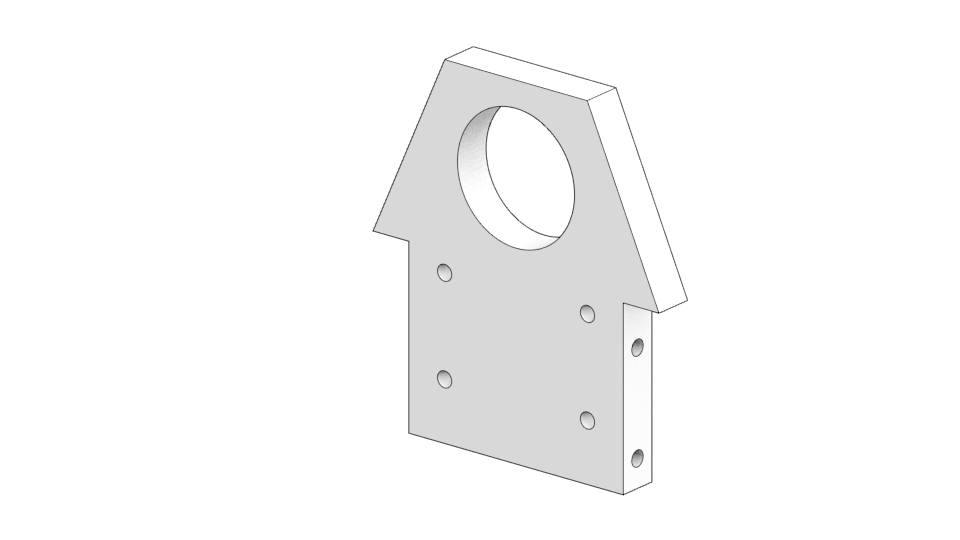
\includegraphics[width=\textwidth]{figures/axis_large.png}
                \caption*{axis large.stl }
        \end{subfigure}
        ~ 
        \begin{subfigure}[b]{0.3\textwidth}
                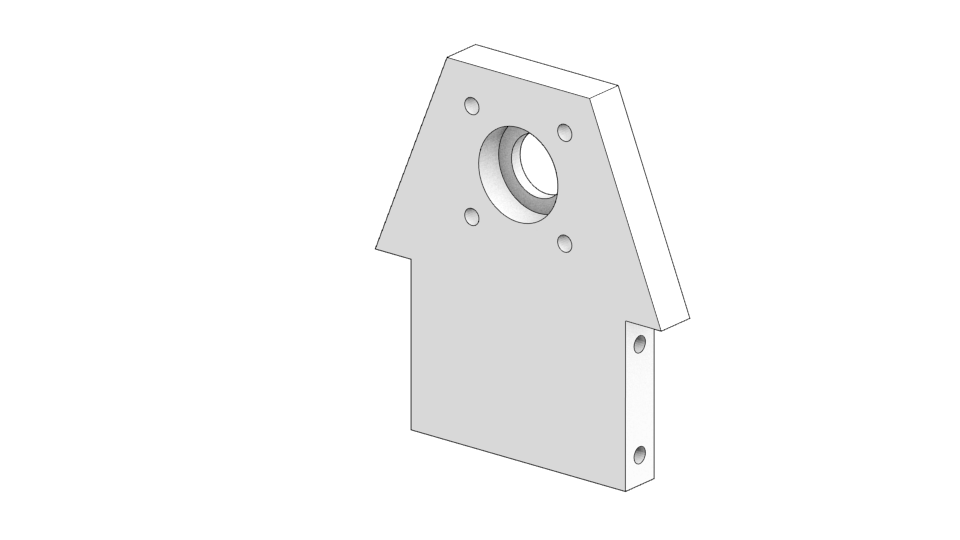
\includegraphics[width=\textwidth]{figures/axis_small.png}
                \caption*{axis small.stl }
        \end{subfigure}
        ~ 
        \begin{subfigure}[b]{0.3\textwidth}
                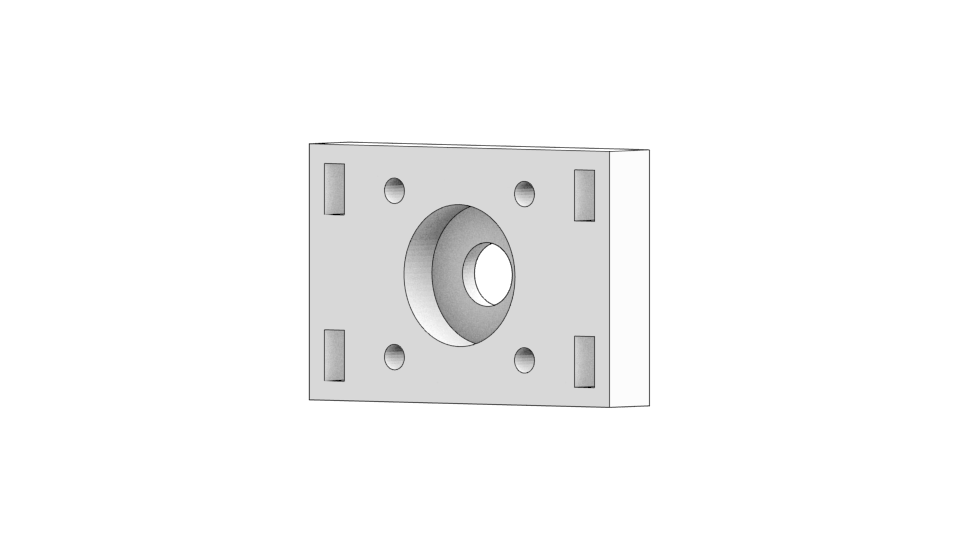
\includegraphics[width=\textwidth]{figures/motor_mount.png}
                \caption*{motor mount.stl }
        \end{subfigure}
\end{figure}

\vspace{0.5cm}

\begin{figure}
        \centering
        \begin{subfigure}[b]{0.3\textwidth}
                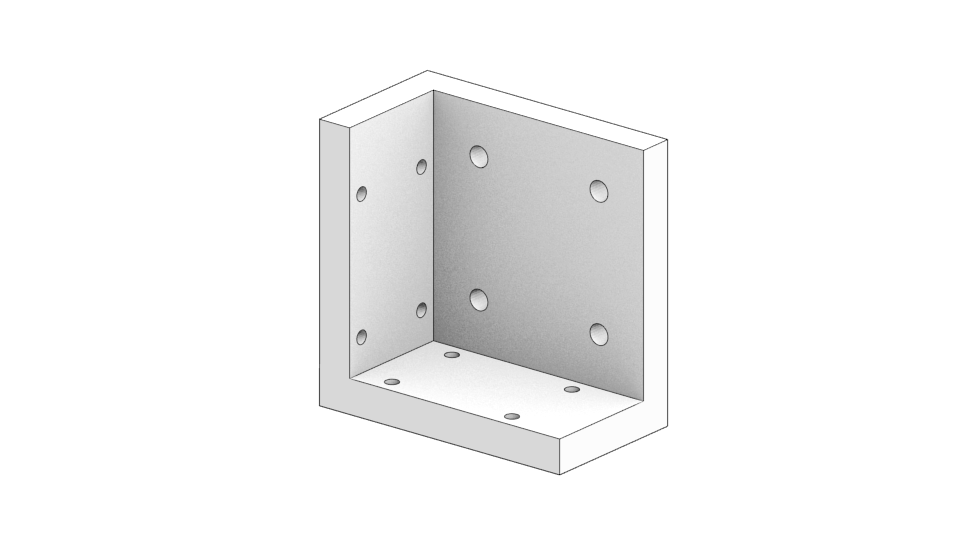
\includegraphics[width=\textwidth]{figures/base.png}
                \caption*{base.stl }
        \end{subfigure}
        ~ 
        \begin{subfigure}[b]{0.3\textwidth}
                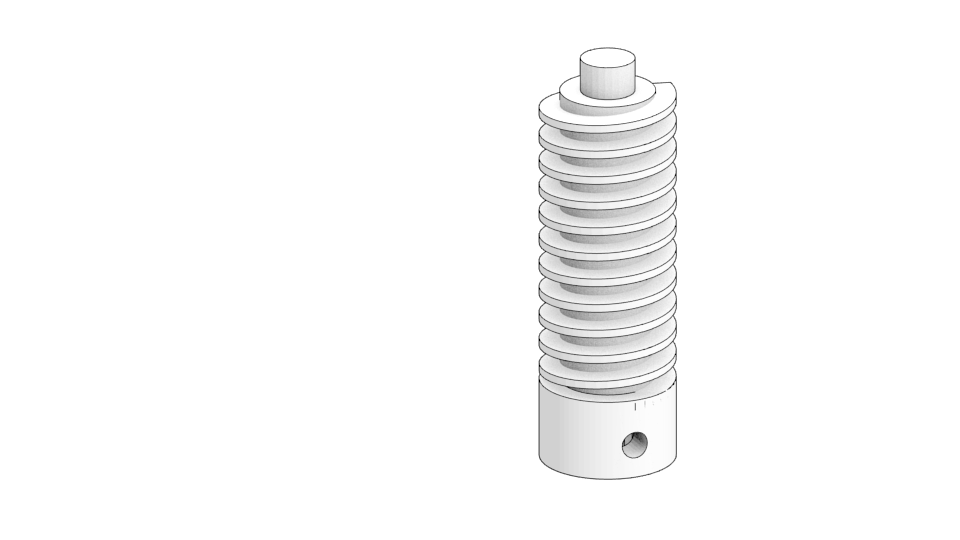
\includegraphics[width=\textwidth]{figures/worm_gear.png}
                \caption*{worm gear.stl }
        \end{subfigure}
        ~ 
        \begin{subfigure}[b]{0.3\textwidth}
                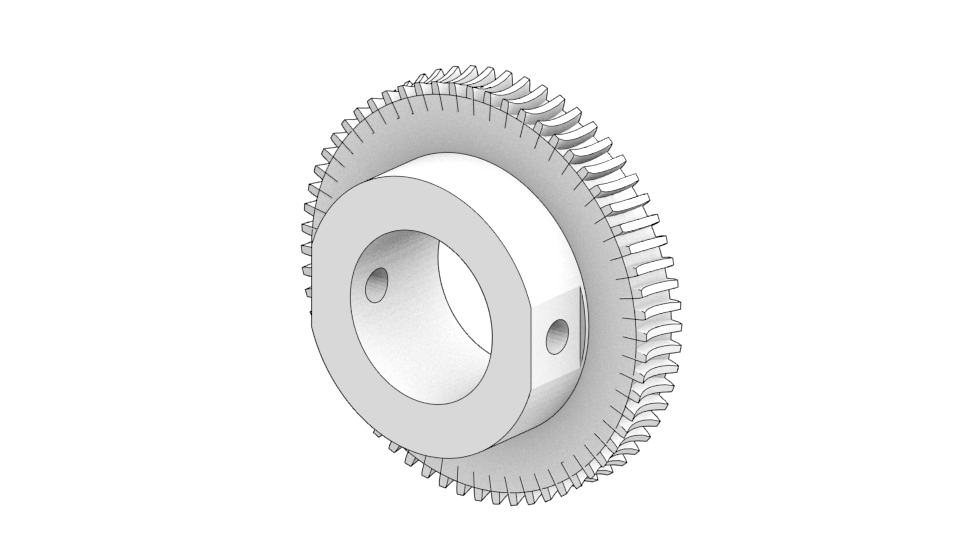
\includegraphics[width=\textwidth]{figures/gear.png}
                \caption*{gear.stl }
        \end{subfigure}
\end{figure}

\vspace{0.5cm}

\begin{figure}
        \centering
        \begin{subfigure}[b]{0.3\textwidth}
                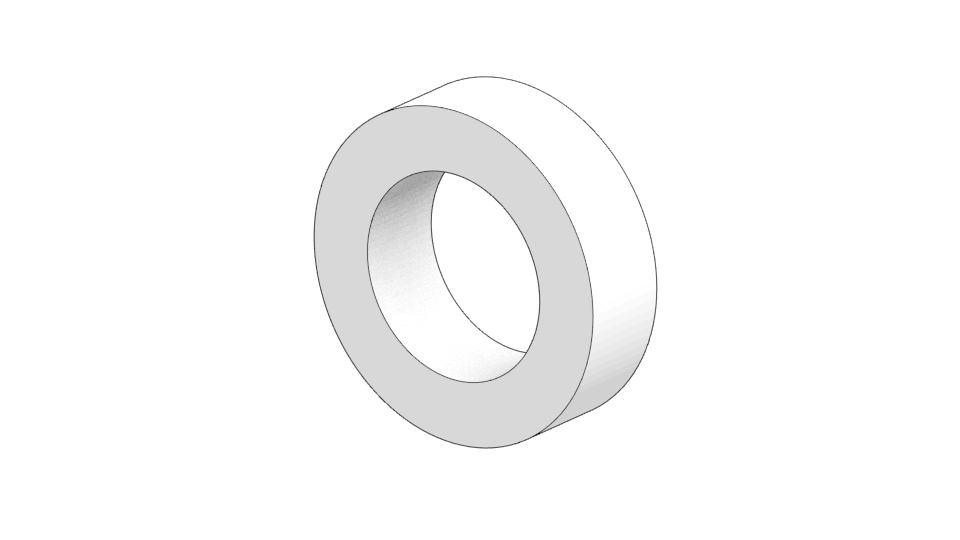
\includegraphics[width=\textwidth]{figures/gear_ring.png}
                \caption*{gear ring.stl }
        \end{subfigure}
        ~ 
        \begin{subfigure}[b]{0.3\textwidth}
                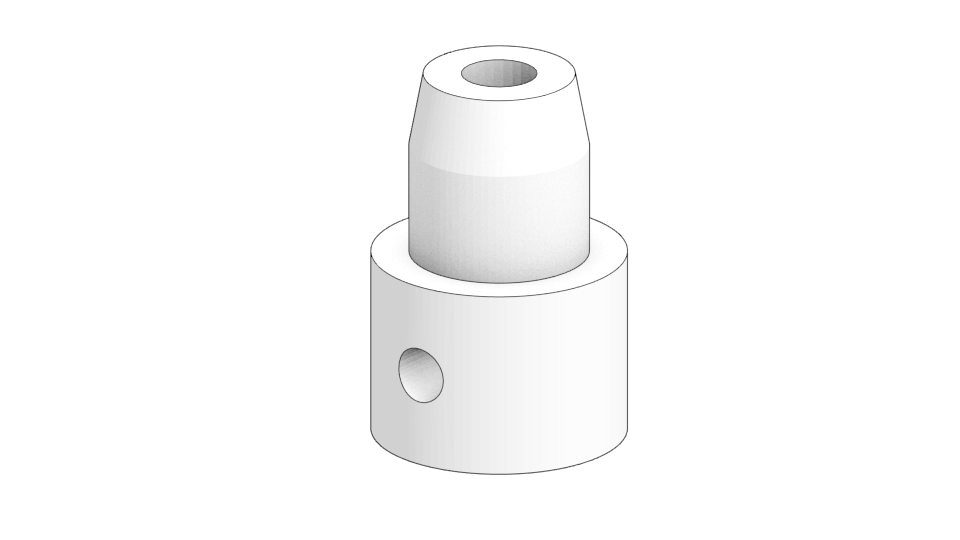
\includegraphics[width=\textwidth]{figures/azimuth_spacer.png}
                \caption*{azimuth spacer.stl }
        \end{subfigure}
        ~ 
        \begin{subfigure}[b]{0.3\textwidth}
                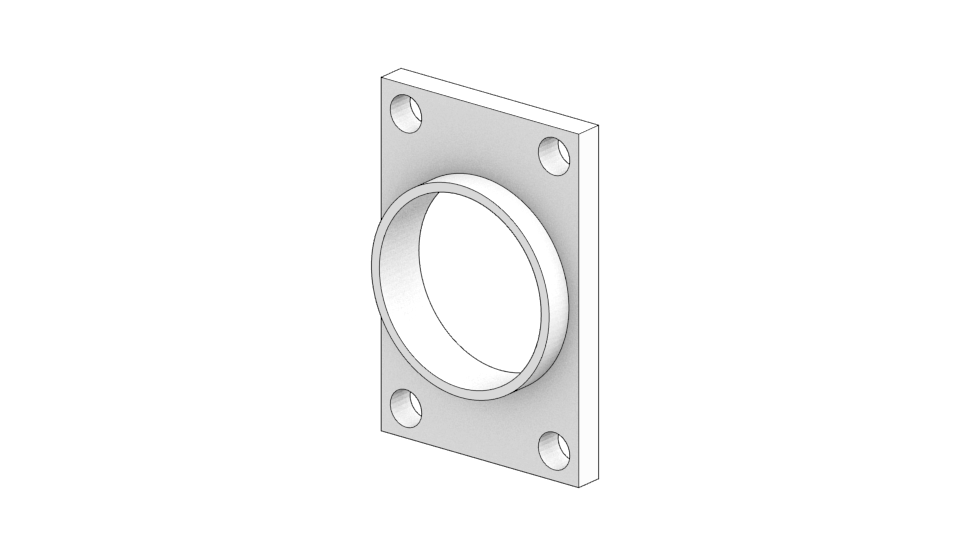
\includegraphics[width=\textwidth]{figures/box_axis_bushing.png}
                \caption*{box axis bushing.stl }
        \end{subfigure}
\end{figure}

\vspace{0.5cm}

\begin{figure}
        \centering
        \begin{subfigure}[b]{0.3\textwidth}
                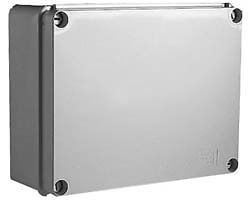
\includegraphics[width=\textwidth]{figures/Box.jpg}
                \caption*{IP56 Box 300x220x120 }
        \end{subfigure}
\end{figure}

\end{document}





